\chapter{Purpose and Organisation}

\section{Introduction}

The technical reference, as you might expect, provides the detail
of the \pharmml specification and aims to provide a definition of the
language in a form that is useful to those developing software tools
that support the language, and reviewers who wish to understand its
fine details.

The reference is organised to first provide background about the design
guidelines and conventions used and then give an annotated description
of the XML Schema definition (both in chapter \ref{techchap:design}).
Then an enumeration of the language's rules is given (in chapter \ref{chapter:validation})

\section{How is \pharmml Defined?}

The normative definition of \pharmml consists of two parts. First is
the XML Schema definition. This describes the syntax of the XML
document and defines some semantic rules such as constraints on
permitted attribute values (enumerations) and the uniqueness of some
identifiers. In order to be valid \pharmml, an XML document must conform to
this schema definition. The XML Schema definition files are
available with this specification and should be regarded as the
definitive authority. For convenience we provide a documented form of
the schema definition in chapter \ref{techchap:design}, but if there
are any discrepancies between these, then the version in the file should
be regarded as definitive.

Most of the semantic rules in \pharmml are \emph{not} captured by the XML
Schema definition, so the second part of the normative definition
is provided by the rules in chapter \ref{chapter:validation}. The rules
are enumerated to allow validating tools to conveniently refer to them
and also to make them clear. The rules specified here are definitive
and take precedence over sources such as software implementations.


\chapter{The XML Schema Definition}
\label{techchap:design}
\label{chap:design}

\section{Design Guidelines}

In designing the XML Schema definition of \pharmml we adopted a number
of design and naming conventions. These were based on a number of best
practise recommendations\footnote{\url{http://alturl.com/jdmkn}}\textsuperscript{,}\footnote{\url{http://www.xml.com/pub/a/2002/11/20/schemas.html}}
and we have tried to be consistent in their application. Unless
specifically documented a deviation from these guidelines is an error on
our part.

%short url: http://alturl.com/jdmkn
% equiv to: http://www.summa-tech.com/blog/2009/11/07/ten-practical-recommendations-for-designing-and-building-highly-reusable-xml-schemas/

\subsection{XML Schema Compliance}

\pharmml is defined using version 1.0 of the XML Schema\footnote{\url{http://www.w3.org/TR/xmlschema-1/}}.

\subsection{Naming Conventions}

Obviously the XML Schema has rules about how names can be defined, but on
top of these rules we have adopted the following conventions:

\begin{itemize}
\item Names should, wherever possible be, be descriptive of the named
  component's purpose, and acronyms should be avoided.
\item Names should be in English with British English spellings.
\item Names should not be excessively long. Especially names used very
  frequently as they may clutter the XML and unnecessarily bloat the
  size of the resulting XML documents.
\item Element names should be capitalised and use camel case to
  delineate words.
\item Attribute names should start with a lowercase character and use
  camel case to delineate words.
\item Enumerations should follow the convention used for attributes.
\end{itemize}

\subsection{Design Pattern}

We adopted the Venetian Blind design
pattern\footnote{\url{http://www.oracle.com/technetwork/java/design-patterns-142138.html}}
for \pharmml. In this pattern all non-global XML Elements are
defined using a complex type. Complex types were inherited using
extension rather than restriction. Typically we tried to reduce the
number of global XML Elements to make identification of the top level
element easier (in cases where there was a single preferred top-level
element).

The benefit of this approach is that it maximises reuse and extension
of the schema by allowing other schemas to reuse or extend the complex
types. This is at the expense of cluttering the design with a surfeit
of complex type definitions.

\subsection{Namespaces}

The domain name \url{pharmml.org} has been reserved for use by
\pharmml. Consequently we use this domain name in all the namespaces
associated with \pharmml.

There are a number of possible strategies for defining
namespaces\footnote{\url{http://www.ibm.com/developerworks/library/x-namcar/index.html}}
and no definitive best practise. However, we have followed the W3C
conventions\footnote{\url{http://www.w3.org/Provider/Style/URI}} and
used the following form:
\begin{verbatim}
http://pharmml.org/Year/Month/Resource
\end{verbatim}
Here the year and month define when the URL was created and the
\emph{Resource} provides a short, but descriptive name of the purpose
of the schema.

\subsection{Elements}

Elements should always be qualified by a namespace. This corresponds
to the XML Schema declaration: \verb|elementFormDefault="qualified"|.

\subsection{Attributes}

Default attributes effectively change the structure of the DOM from
that described by the XML itself. This can cause problems with
validation and result in difficult to track
errors\footnote{ref}. For these reasons the use of default attribute
values is forbidden.

Attributes should never be qualified by a
namespace\footnote{\url{http://www.xml.com/pub/a/2002/11/20/schemas.html?page=3}}. This
corresponds to the XML Schema declaration
\verb|attributeFormDefault="unqualified"|.

\subsection{Elements vs.\@ Attributes}

It is a common dilema in design XML documents: when do I use an
element and when an attribute? In this schema design we have tried to
follow the advice provided in an IBM technical
document\footnote{\url{http://http://www.ibm.com/developerworks/xml/library/x-eleatt/index.html}}. The
advice can be summarised as follows:

\begin{description}
\item[Principle of core content] Briefly data or core content should
  be held in elements and metadata should be in attributes.
\item[Principle of structured information] If the information needs to
  be structured then it should be represented by an element. If it is
  atomic then us an attribute.
\item[Principle of readability] If the information is intended to be
  read and understood by a person then use elements. If it is intended
  to be used by a machine then use attributes.
\item[Principle of element/attribute binding] If the information to be
  represented can be modified by another attribute then use an element
  to represent it.
\end{description}

These rules are to some extent a matter of judgement and in some cases
there are marginal cases. The names of parameters, variables and other
symbols used in \pharmml are a case in point. The names for such
symbols have meaning for a modeller, but they are also used
computationally. In addition, variable names can have to forms, a
computer friendly form such as \texttt{omega\_V} and a mathematical
form such as $\omega_V$. Currently \pharmml only handles the latter
form, and although this is a computational name it is also commonly
used by modellers. Our solution has been to treat the symbol name as
an element that can in the future be extended to handle a mathematical
form of the variable, but with the computation name given as an
attribute. For example:

\begin{xmlcode}
<Variable symbID="pV" symbolType="scalar" >
  <ct:Symbol>pop_V</Symbol>
</Variable>
\end{xmlcode}

In the above case the \xelem{ct:Symbol} element is optional so it is
only provided if the displayed name of the symbol is
required.

\subsection{Keys and Key References}

We use the XML Schema key and keyref mechanisms only. ID and IDREF
types should not be used\footnote{\url{http://www.xml.com/pub/a/2002/11/20/schemas.html?page=3\#identity_constraints}}.

\subsection{Versioning Strategy}

\pharmml will change over time and indeed we have described the
versioning strategy for \pharmml earlier in this document (section
\ref{intro:versioning} on page \pageref{intro:versioning}). While this
makes clear how we anticipate the specification document to change,
what we also need to accommodate are changes to the XML Schema
definition that such change implies.

Unfortunately there is no definitive solution for versioning XML
Schema definitions, but we are following the conventions described
elsewhere\footnote{\url{http://www.xfront.com/Versioning.pdf}}. In particular we
will do the following:
\begin{enumerate}
\item Use the \xatt{version} attribute in the XML Schema definition to
  define the current version of the schema.
\item Add a version attribute in the top-most elements of the instance
  document indicating what version they were compliant with, when they
  were last updated.
\item Rely on the \pharmml validator to ensure that the version of the
  instance document and XML Schema definition are compatible.
\item The namespace URL will only change if there is a significant
  change in the symbols defined in the namespace or if the meaning of
  a significant proportion has been redefined.
\end{enumerate}

\section{XML Schema Organisation}

\pharmml is a large language and the XML Schema definition is
correspondingly large too. Fortunately, the language is naturally
organised into three sections (see chapter
\ref{chap:lang-overview}): Model Definition, Trial Design, and
Modelling Steps, which provides us with a convenient way to modularise
the XML Schema definition. In addition, we have two components, which
are also naturally independent of the core \pharmml specification: the
definition of both mathematical expressions and probability
distributions. Using these natural divisions, we split the \pharmml XML Schema
definition into the following xsd files.

\begin{center}
\footnotesize
\begin{tabular}[t]{l@{\hspace{1mm}} l@{\hspace{1mm}} p{5.9cm}}\toprule
File Name & Namespace URI & Description\\\midrule
pharmml.xsd & http://www.pharmml.org/2013/03/PharmML & The overall
\pharmml definition that includes all the other components.\\
modelDefinition.xsd & http://www.pharmml.org/2013/03/ModelDefinition &
Defines the model definition section.\\
trialDesign.xsd & http://www.pharmml.org/2013/03/TrialDesign & Defines
the trial design section.\\
modellingSteps.xsd & http://www.pharmml.org/2013/03/ModellingSteps &
Defines the modelling steps section.\\
commonTypes.xsd & http://www.pharmml.org/2013/03/CommonTypes & Defines
the type definitions and structures common to the above
schema definitions.\\
dataset.xsd & http://www.pharmml.org/2013/08/Dataset & Defined the
dataset and related structures that is used in the trial design and
modelling steps to represent tabular data.\\
maths.xsd & http://www.pharmml.org/2013/03/Maths & Defines the
representation of mathematical expressions.\\
UncertML30.xsd & http://www.uncertml.org/3.0 & Defines
the probability distributions provided by \pharmml.\\\bottomrule\\
\end{tabular}
\end{center}

Note that a \pharmml document must be compliant with the pharmml.xsd
definition, which includes all the other components. The other schema
definitions should not be used independently to validate a \pharmml
document.

%\clearpage
\chapter{Schema Description}
\label{chap:schema-defn}

In this chapter the detailed documentation of the XML
Schemas used to define \pharmml is included. All the schemas except
the \uncertml schema is included. \uncertml is maintained separately
from \pharmml and for more information you should go to
\url{http://www.uncertml.org}.

%\includepdf[pages=6-,pagecommand={},picturecommand={\color{white}\put(300,42){\circle*{10}}}]{reference/moml}

%\section{\pharmml}
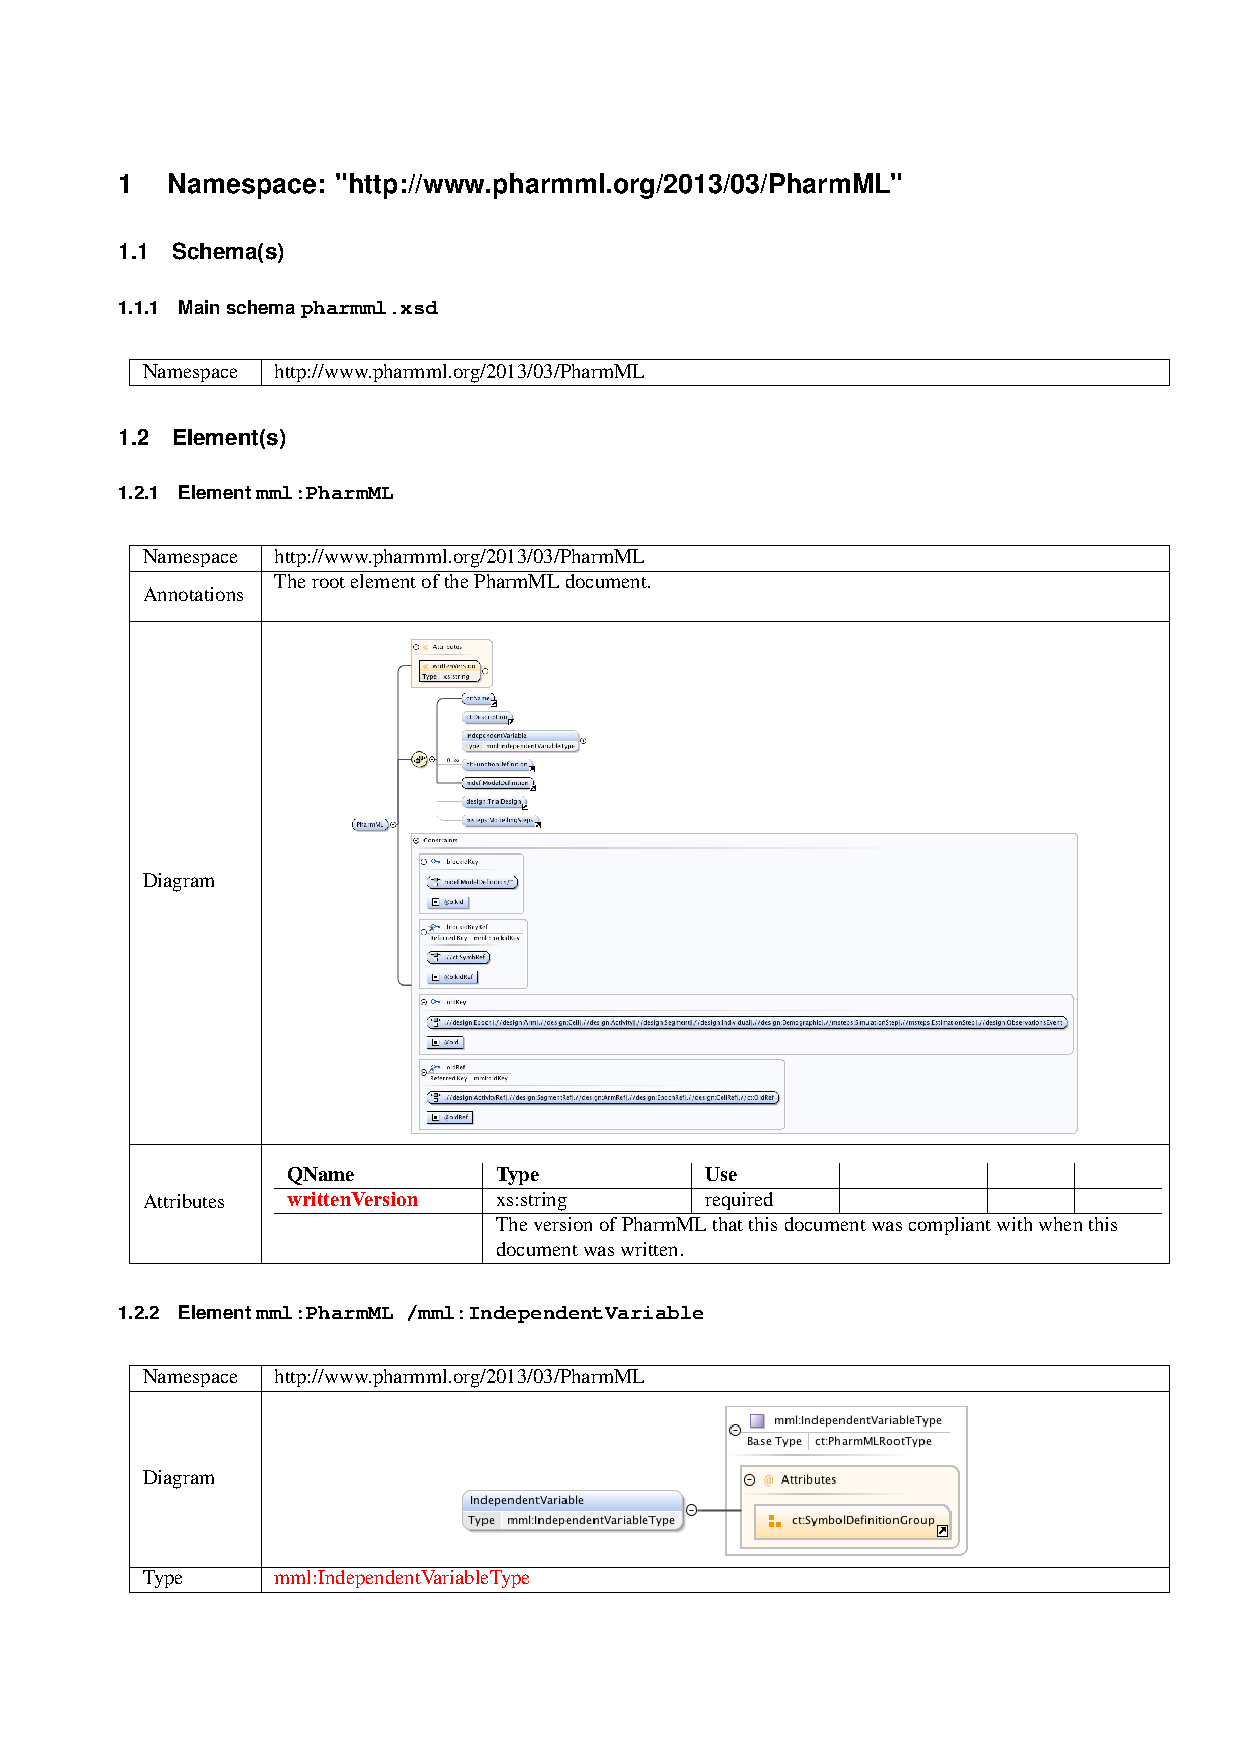
\includepdf[pages=1,pagecommand={\thispagestyle{plain}\section{\pharmml}},offset=0
-1cm]{reference/pharmml}
\includepdf[pages=2-,pagecommand={\thispagestyle{plain}}]{reference/pharmml}

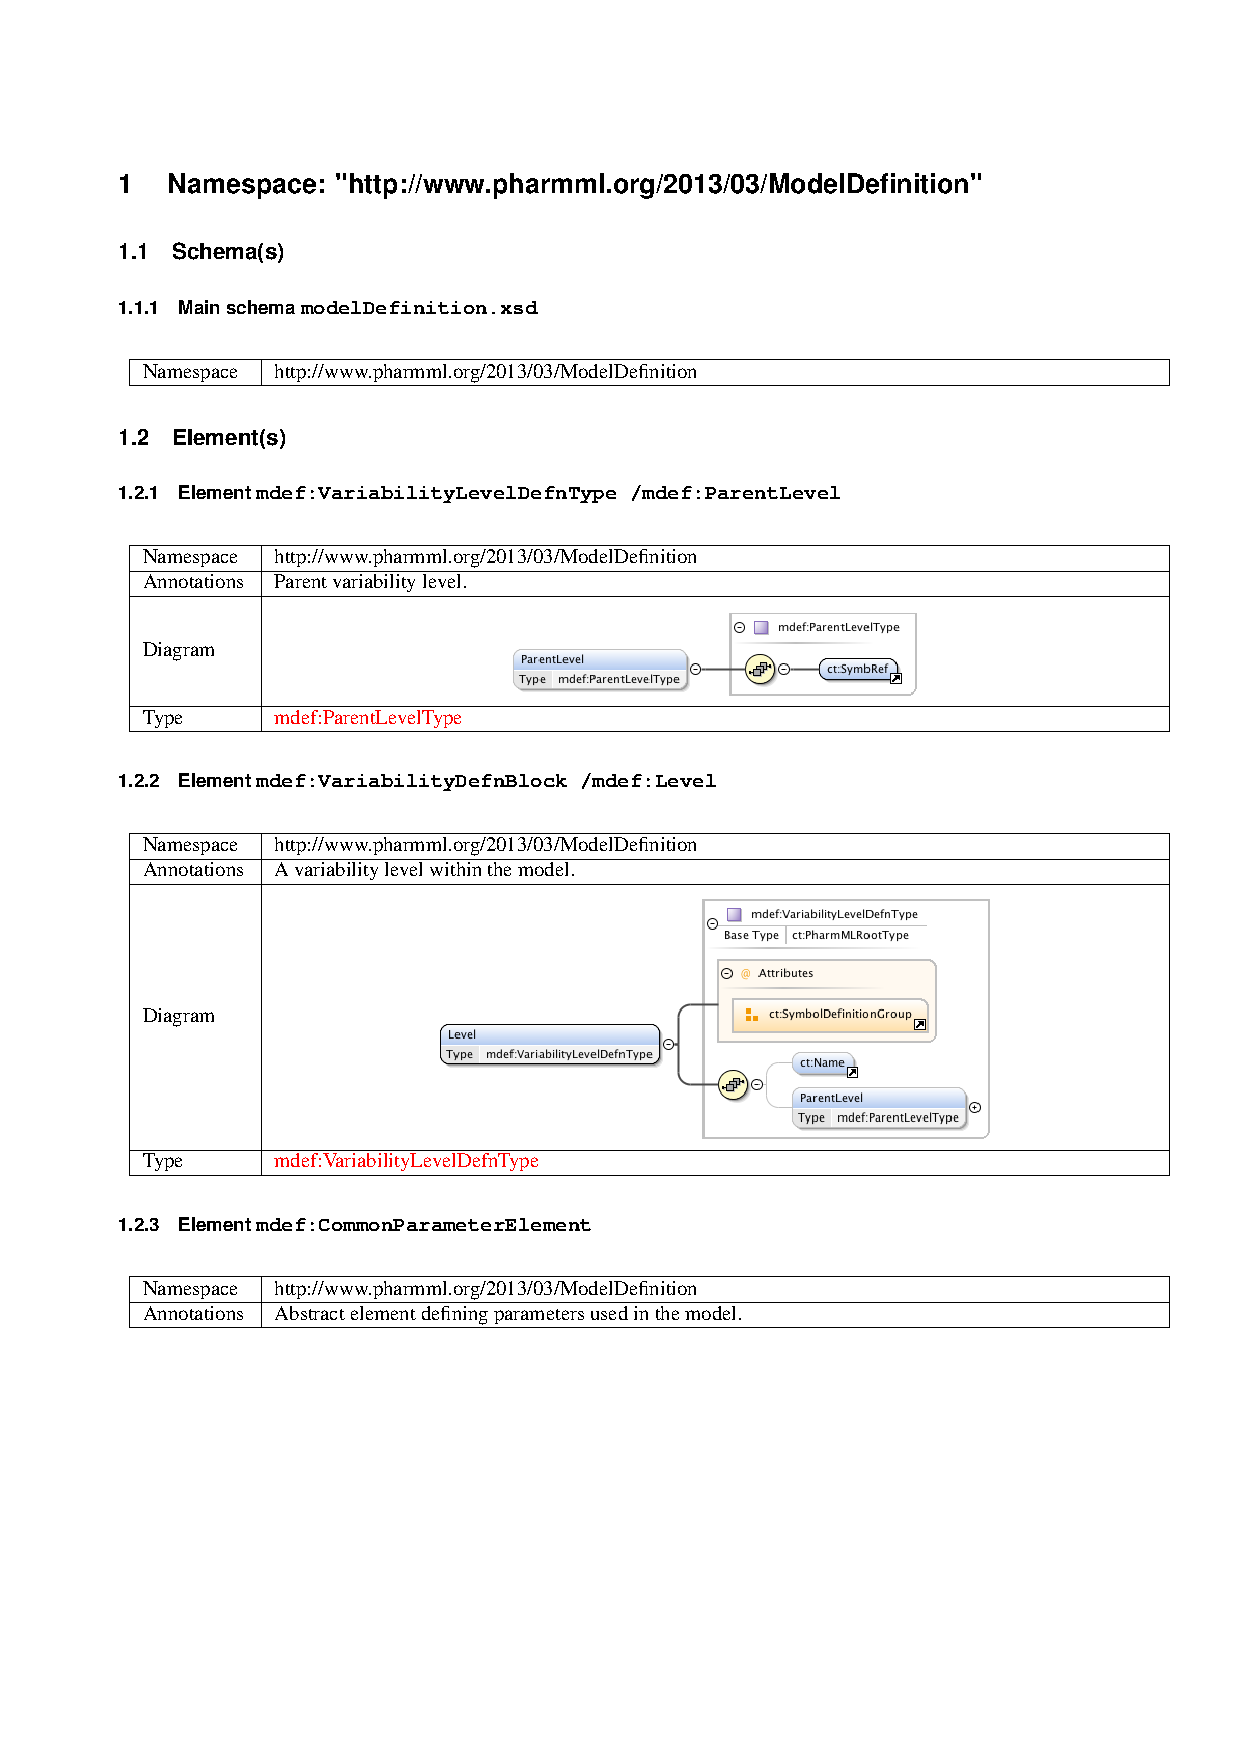
\includepdf[pages=1,pagecommand={\thispagestyle{plain}\section{Model Definition}},offset=0
-1cm]{reference/modelDefinition}
\includepdf[pages=2-,pagecommand={\thispagestyle{plain}}]{reference/modelDefinition}

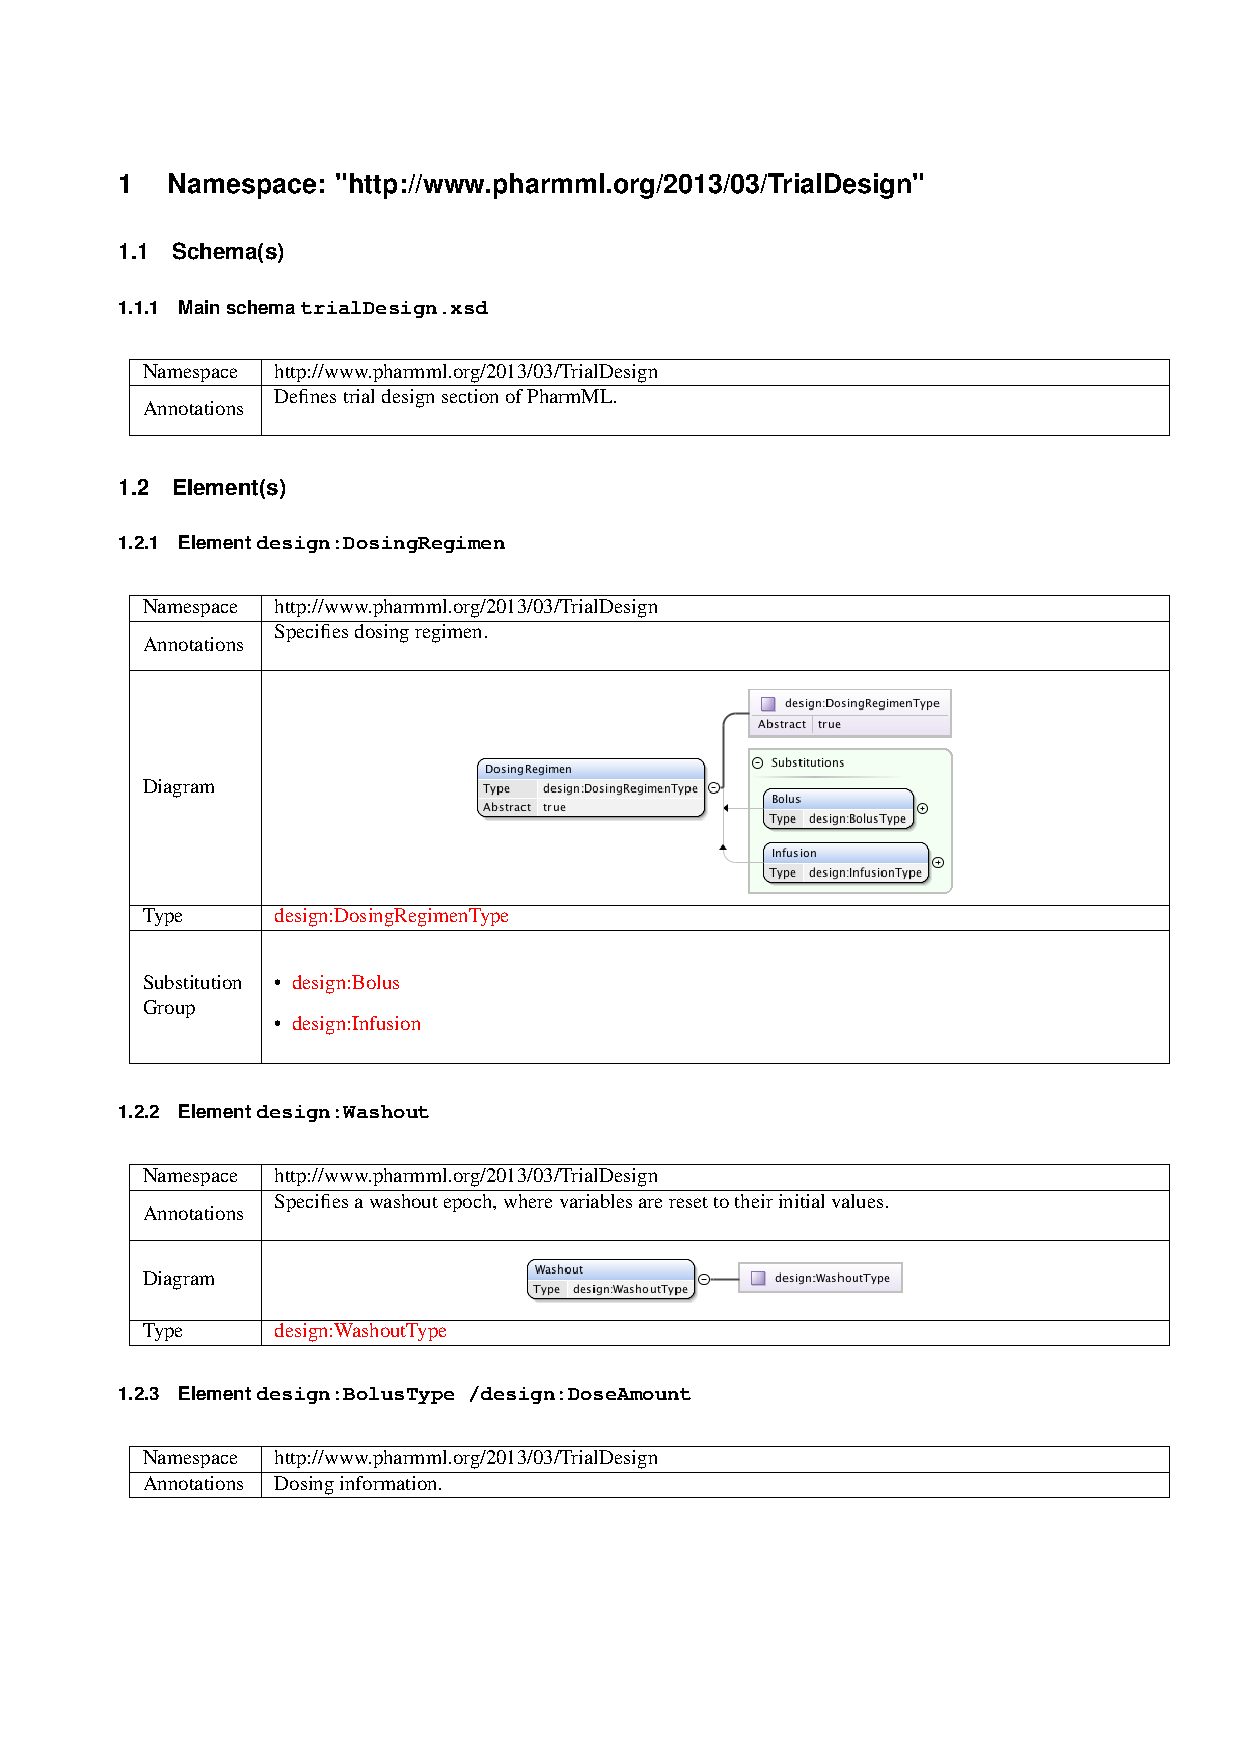
\includepdf[pages=1,pagecommand={\thispagestyle{plain}\section{Trial Design}},offset=0
-1cm]{reference/trialDesign}
\includepdf[pages=2-,pagecommand={\thispagestyle{plain}}]{reference/trialDesign}

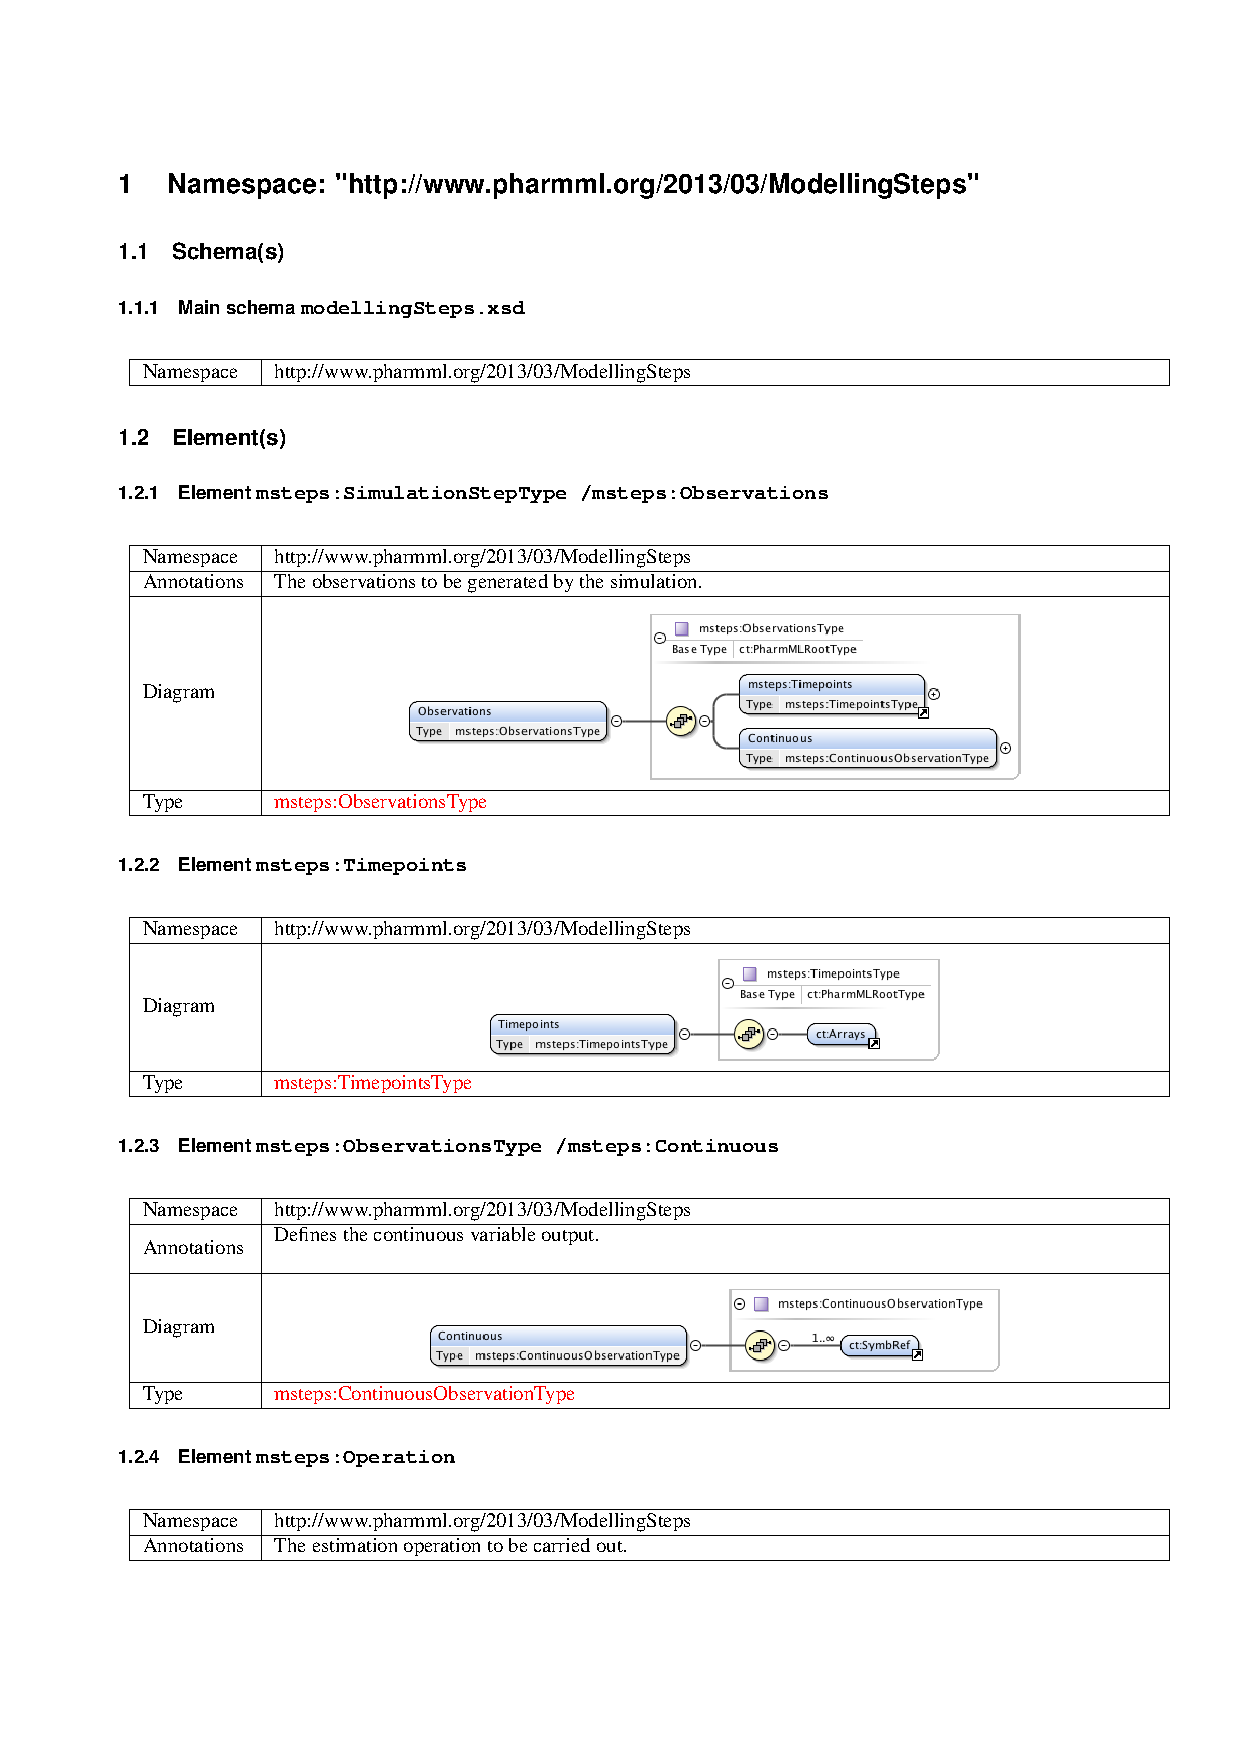
\includepdf[pages=1,pagecommand={\thispagestyle{plain}\section{Modelling
  Steps}},offset=0 -1cm]{reference/modellingSteps}
\includepdf[pages=2-,pagecommand={\thispagestyle{plain}}]{reference/modellingSteps}

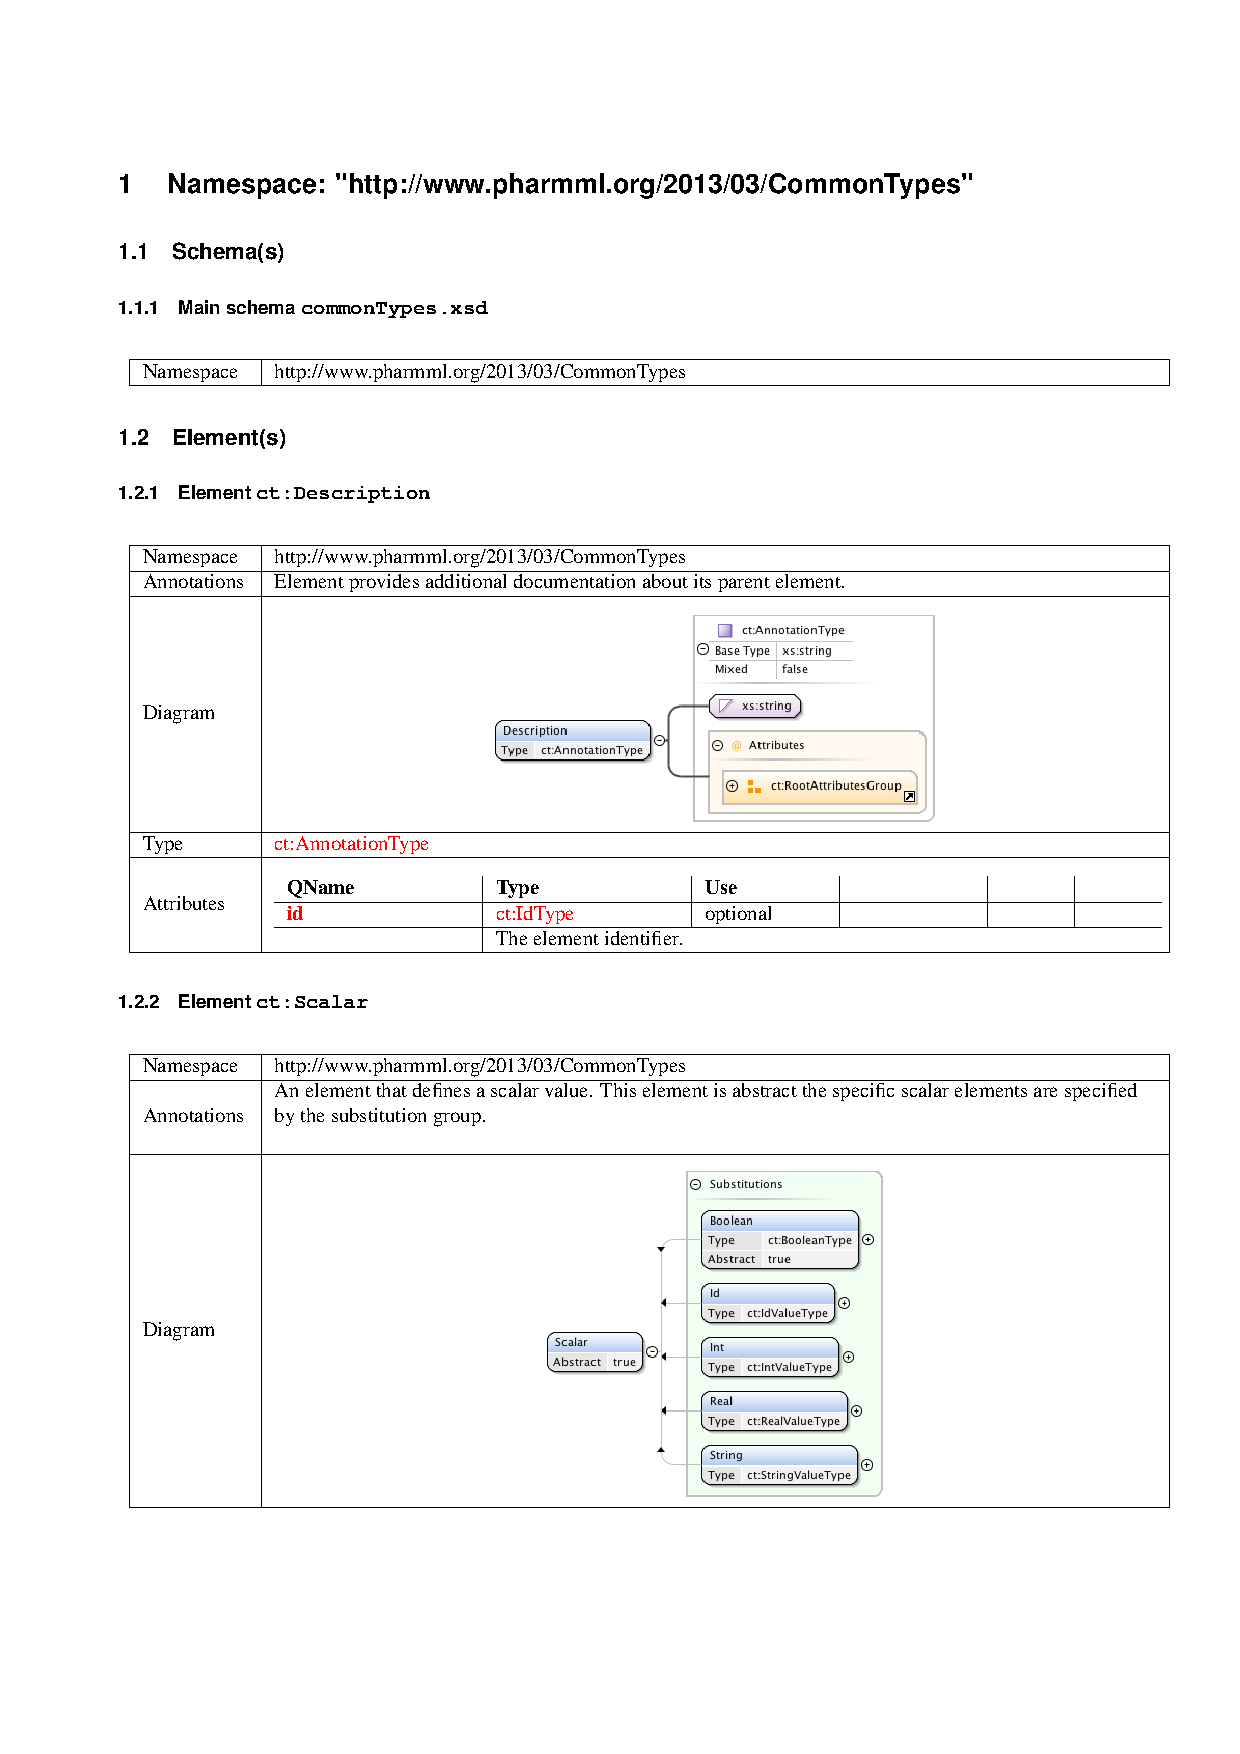
\includepdf[pages=1,pagecommand={\thispagestyle{plain}\section{Common Types}},offset=0
-1cm]{reference/commonTypes}
\includepdf[pages=2-,pagecommand={\thispagestyle{plain}}]{reference/commonTypes}

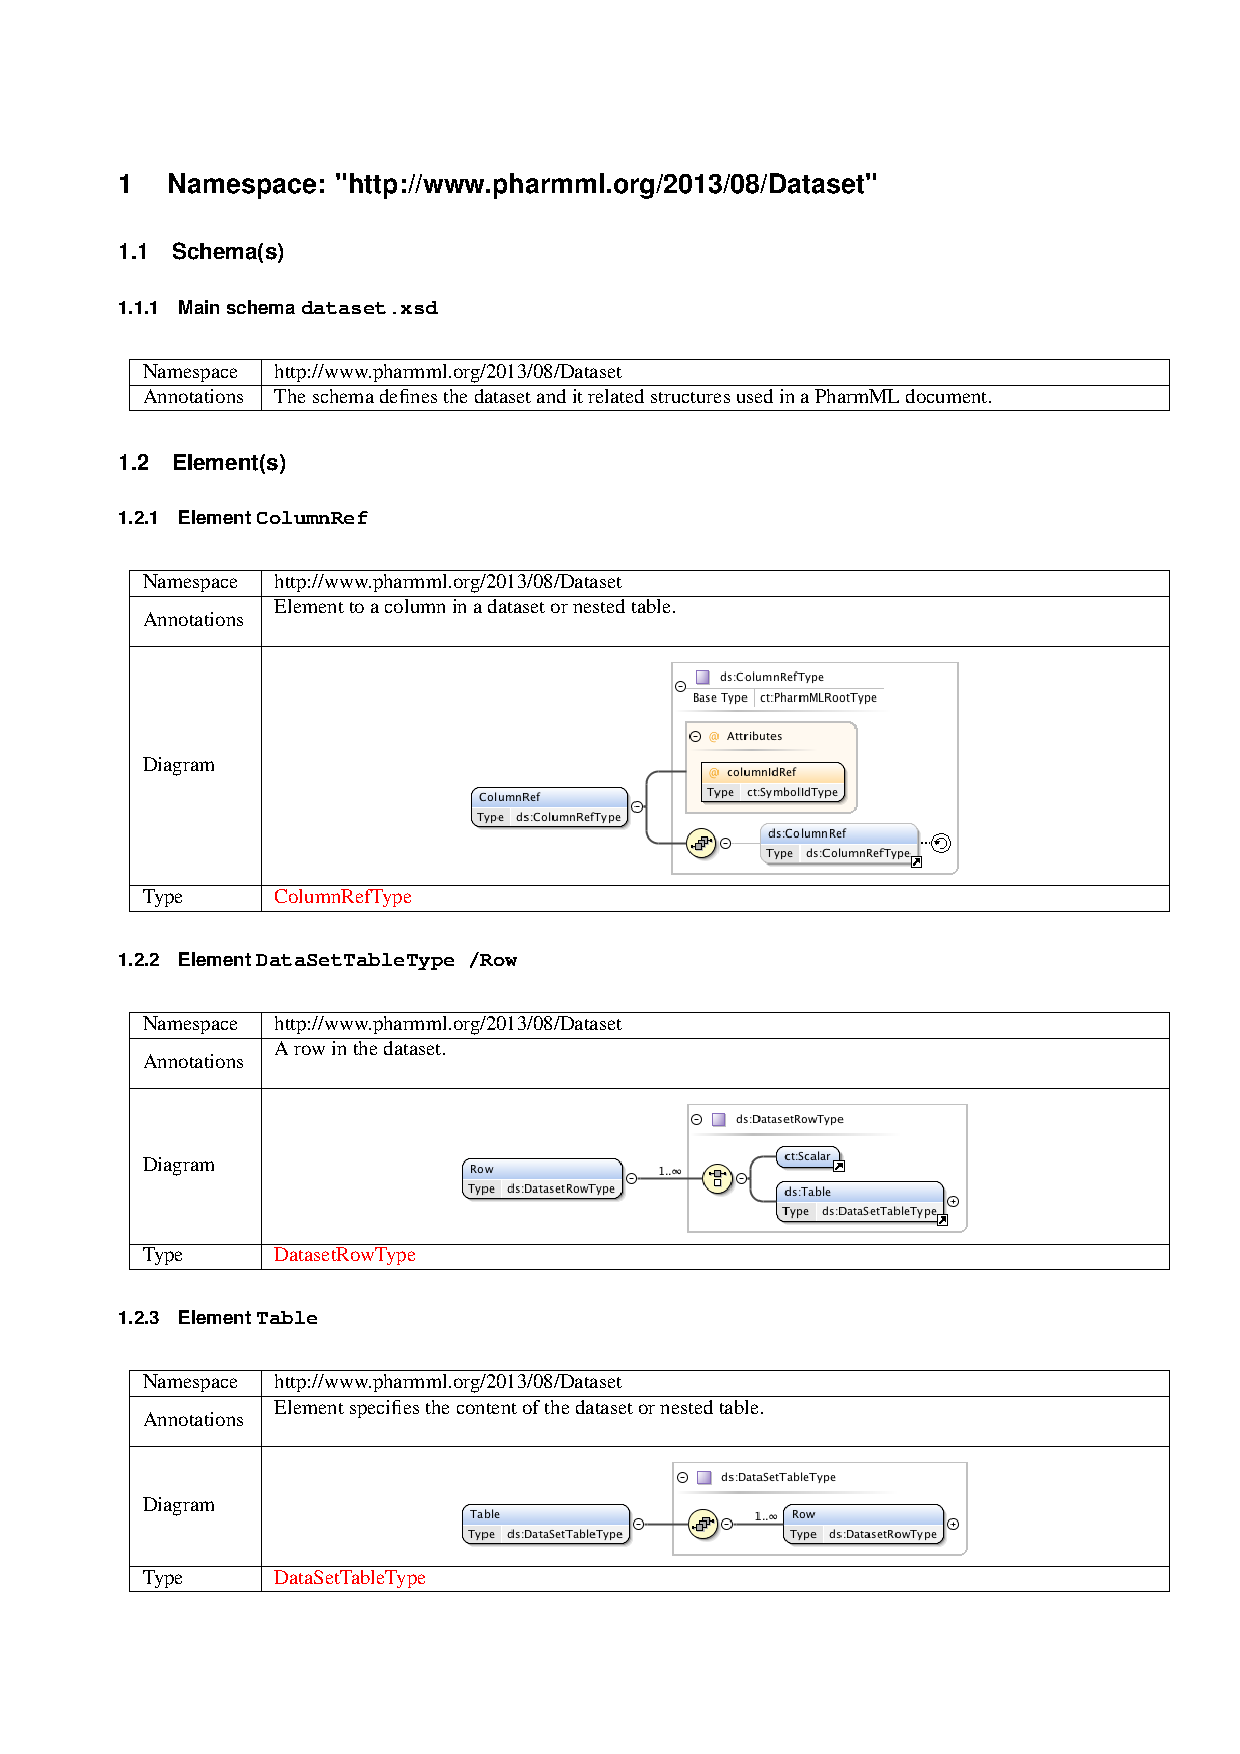
\includepdf[pages=1,pagecommand={\thispagestyle{plain}\section{Dataset}},offset=0
-1cm]{reference/dataset}
\includepdf[pages=2-,pagecommand={\thispagestyle{plain}}]{reference/dataset}

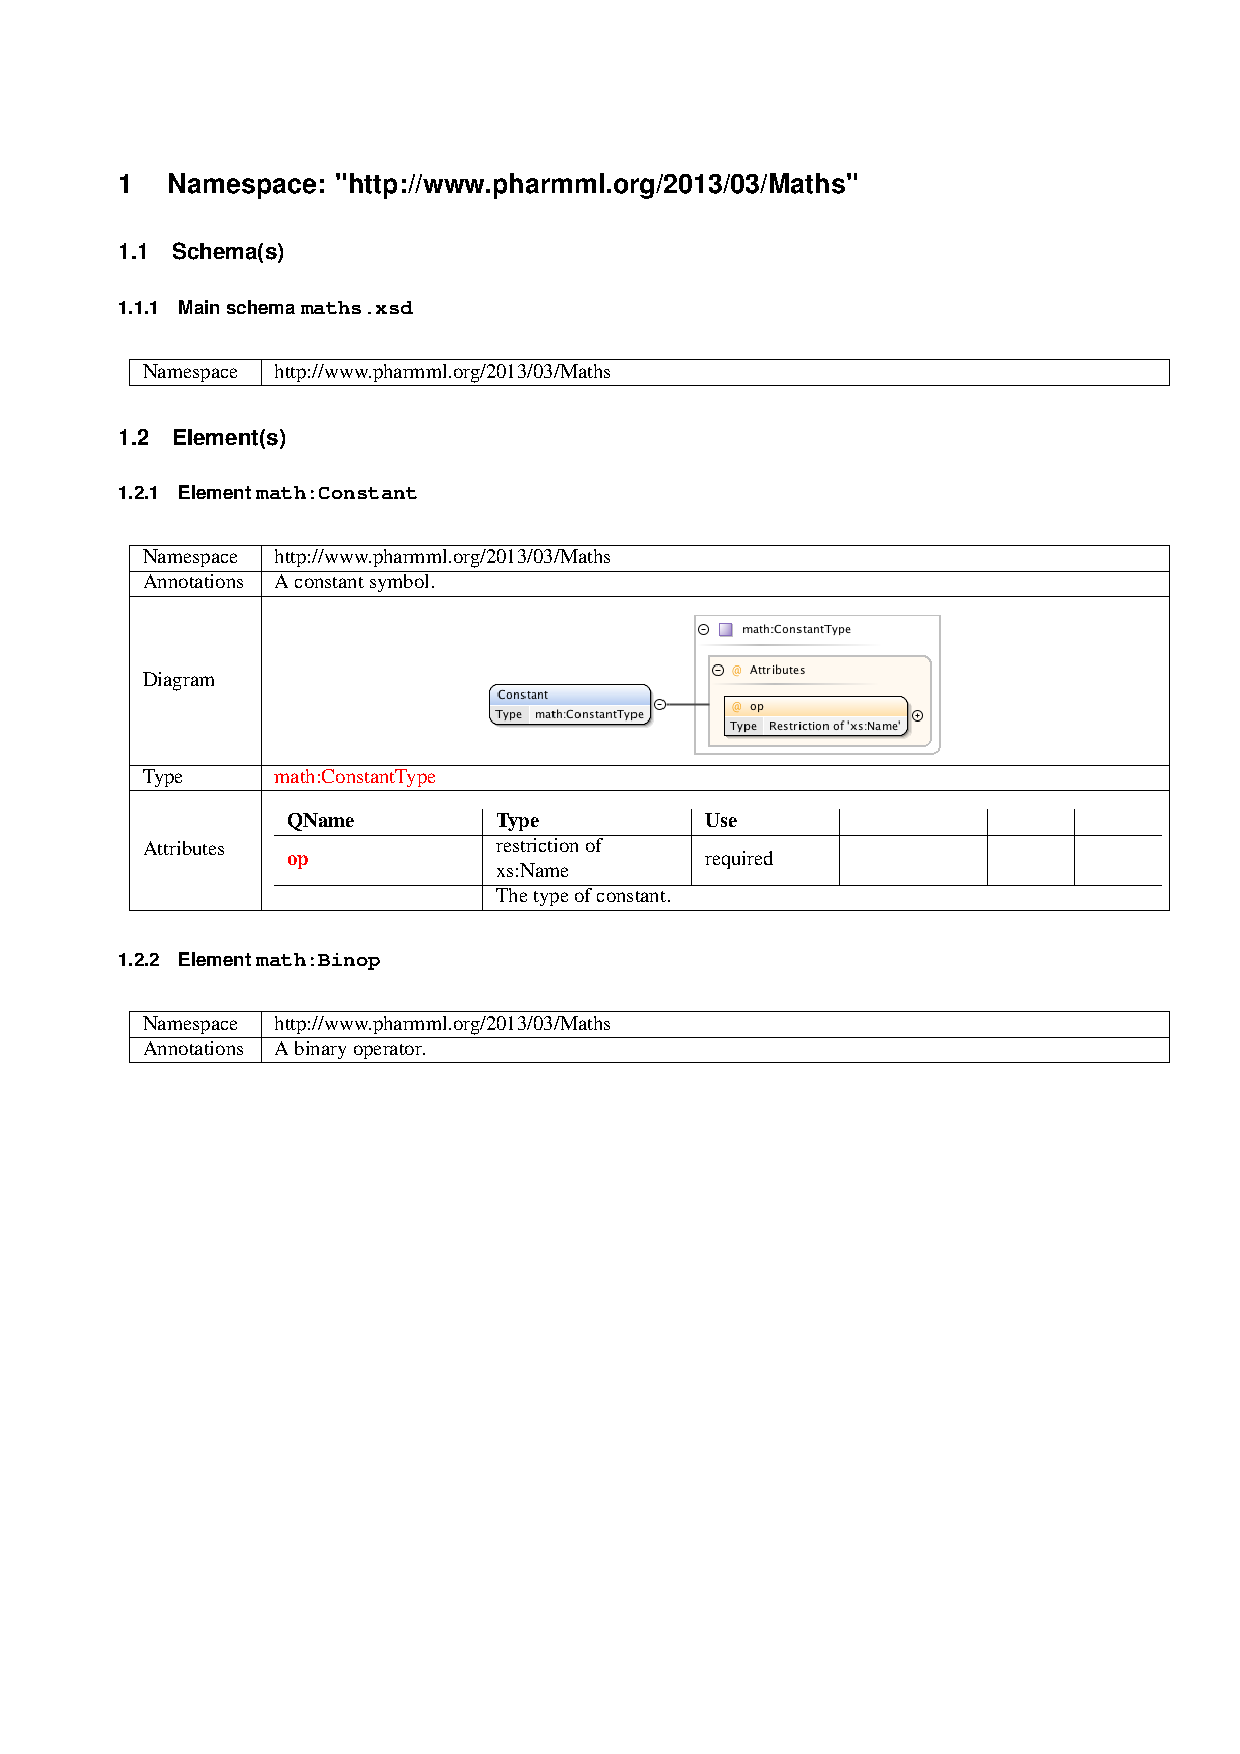
\includepdf[pages=1,pagecommand={\thispagestyle{plain}\section{Maths}},offset=0
-1cm]{reference/maths}
\includepdf[pages=2-,pagecommand={\thispagestyle{plain}}]{reference/maths}

